% ------------------------------------------------------------------------
% ------------------------------------------------------------------------
% abnTeX2: Modelo de Trabalho Academico (tese de doutorado, dissertacao de
% mestrado e trabalhos monograficos em geral) em conformidade com 
% ABNT NBR 14724:2011: Informacao e documentacao - Trabalhos academicos -
% Apresentacao
% ------------------------------------------------------------------------
% ------------------------------------------------------------------------

\documentclass[
	% -- opções da classe memoir --
	12pt,				% tamanho da fonte
	openright,			% capítulos começam em pág ímpar (insere página vazia caso preciso)
	%twoside,			% para impressão em verso e anverso. Oposto a oneside
	oneside,
	a4paper,			% tamanho do papel. 
	% -- opções da classe abntex2 --
	%chapter=TITLE,		% títulos de capítulos convertidos em letras maiúsculas
	%section=TITLE,		% títulos de seções convertidos em letras maiúsculas
	%subsection=TITLE,	% títulos de subseções convertidos em letras maiúsculas
	%subsubsection=TITLE,% títulos de subsubseções convertidos em letras maiúsculas
	% -- opções do pacote babel --
	english,			% idioma adicional para hifenização
	french,				% idioma adicional para hifenização
	spanish,			% idioma adicional para hifenização
	brazil				% o último idioma é o principal do documento
	]{abntex2}

% ---
% Pacotes básicos 
% ---
\usepackage{lmodern}			% Usa a fonte Latin Modern			
\usepackage[T1]{fontenc}		% Selecao de codigos de fonte.
\usepackage[utf8]{inputenc}		% Codificacao do documento (conversão automática dos acentos)
\usepackage{lastpage}			% Usado pela Ficha catalográfica
\usepackage{indentfirst}		% Indenta o primeiro parágrafo de cada seção.
\usepackage{color}				% Controle das cores
\usepackage{graphicx}			% Inclusão de gráficos
\usepackage{microtype} 			% para melhorias de justificação
% ---
		
% ---
% Pacotes adicionais, usados apenas no âmbito do Modelo Canônico do abnteX2
% ---
\usepackage{lipsum}				% para geração de dummy text
% ---

% ---
% Pacotes de citações
% ---
\usepackage[brazilian,hyperpageref]{backref}	 % Paginas com as citações na bibl
\usepackage[alf]{abntex2cite}	% Citações padrão ABNT

% define o caminho das imagens
\graphicspath{{Imagens/}}

% --- 
% CONFIGURAÇÕES DE PACOTES
% --- 

% ---
% Configurações do pacote backref
% Usado sem a opção hyperpageref de backref
\renewcommand{\backrefpagesname}{Citado na(s) página(s):~}
% Texto padrão antes do número das páginas
\renewcommand{\backref}{}
% Define os textos da citação
\renewcommand*{\backrefalt}[4]{
	\ifcase #1 %
		Nenhuma citação no texto.%
	\or
		Citado na página #2.%
	\else
		Citado #1 vezes nas páginas #2.%
	\fi}%
% ---

% ---
% Informações de dados para CAPA e FOLHA DE ROSTO
% ---
\titulo{Título Provisório da Monografia de\\ Trabalho de Conclusão de Curso}
\autor{Rodrigo Mendonça da Paixão \\ Lucas Teles Agostinho}
\local{São Paulo -- Brasil}
\data{2015}
\orientador{Eduardo Heredia}
%\coorientador{Nome Completo}
\instituicao{%
  Centro Universitário Senac
  \par
  Bacharelado em Ciência da Computação
}
\tipotrabalho{Monografia (Graduação)}
% O preambulo deve conter o tipo do trabalho, o objetivo, 
% o nome da instituição e a área de concentração 
\preambulo{Pré-monografia apresentada na disciplina Trabalho de Conclusão de Curso I, como parte dos requisitos para obtenção do título de Bacharel em Ciência da Computação.}
% ---

% ---
% Configurações de aparência do PDF final

% alterando o aspecto da cor azul
\definecolor{blue}{RGB}{41,5,195}

% informações do PDF
\makeatletter
\hypersetup{
     	%pagebackref=true,
		pdftitle={\@title}, 
		pdfauthor={\@author},
    	pdfsubject={\imprimirpreambulo},
	    pdfcreator={LaTeX with abnTeX2},
		pdfkeywords={abnt}{latex}{abntex}{abntex2}{trabalho acadêmico}, 
		colorlinks=true,       		% false: boxed links; true: colored links
    	linkcolor=blue,          	% color of internal links
    	citecolor=blue,        		% color of links to bibliography
    	filecolor=magenta,      		% color of file links
		urlcolor=blue,
		bookmarksdepth=4
}
\makeatother
% --- 

% --- 
% Espaçamentos entre linhas e parágrafos 
% --- 

% O tamanho do parágrafo é dado por:
\setlength{\parindent}{1.3cm}

% Controle do espaçamento entre um parágrafo e outro:
\setlength{\parskip}{0.2cm}  % tente também \onelineskip

% ---
% compila o indice
% ---
\makeindex
% ---

% ----
% Início do documento
% ----
\begin{document}

% Retira espaço extra obsoleto entre as frases.
\frenchspacing 

% ----------------------------------------------------------
% ELEMENTOS PRÉ-TEXTUAIS
% ----------------------------------------------------------
% \pretextual

% ---
% Capa
% ---
\imprimircapa
% ---

% ---
% Folha de rosto
% (o * indica que haverá a ficha bibliográfica)
% ---
\imprimirfolhaderosto%*
% ---

% ---
% RESUMOS
% ---

% resumo em português
\setlength{\absparsep}{18pt} % ajusta o espaçamento dos parágrafos do resumo
\begin{resumo}
   
 \textbf{Palavras-chaves}: IDS,Rede,Internet
\end{resumo}

% ---
% inserir lista de ilustrações (figuras)
% ---
\pdfbookmark[0]{\listfigurename}{lof}
\listoffigures*
\cleardoublepage
% ---

% ---
% inserir lista de tabelas
% ---
\pdfbookmark[0]{\listtablename}{lot}
\listoftables*
\cleardoublepage
% ---

% ---
% inserir lista de abreviaturas e siglas
% ---
\begin{siglas}
  \item[ABNT] Associação Brasileira de Normas Técnicas
  \item[abnTeX] ABsurdas Normas para TeX
\end{siglas}
% ---

% ---
% inserir o sumario
% ---
\pdfbookmark[0]{\contentsname}{toc}
\tableofcontents*
\cleardoublepage
% ---

% ----------------------------------------------------------
% ELEMENTOS TEXTUAIS 
% ----------------------------------------------------------
\textual

% ----------------------------------------------------------
% Capitulo 1
% ----------------------------------------------------------
\chapter[Introdução]{Introdução}
%\addcontentsline{toc}{chapter}{Introdução}
% ----------------------------------------------------------
Detecção de intrução é uma forma de monitorar eventos em um sistema de computador ou uma rede de computadores,
e analisar possiveis incidentes,utilizando de politicas ou uso pratico.

\section{Motivação}

Eventos de intrução estão ficando cada vez mais comuns, por que,
empresas e pessoas dependem cada vez mais da infra estrutura computacional e estaão cada vez mais conectados a internet para realizar suas tarefas, este crescimento é exponencial, existindo um risco de estar conectado a todo estante desta forma, 
a preocupação que vem crescendo juntamente a esta necessidade é relativo a segurança da informação.
Mesmo existindo grande esforço para prover segurança neste ambiente, o numero e complexidade de eventos relacionados a quebra de segurança continua crescendo. Pode ser visto pelos reportes feitos ao CERT (Computer Emergency Response Team) até o ano de 2014.
\begin{figure}[!htb]
     \centering
     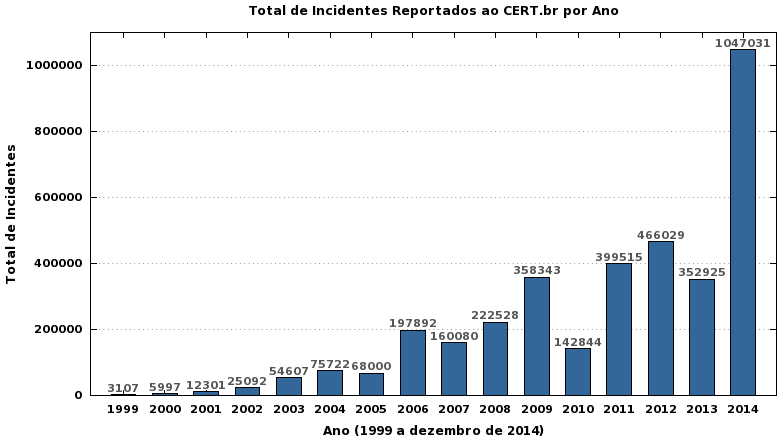
\includegraphics[scale=0.5]{Imagens/IntroGraf.png}
     \caption{Incidentes ano a ano}
\end{figure}

Com esses incidentes ficando cada vez mais comuns, é necessario investir em sistemas de detecção de intrusão e segurança computacional.
O trabalho desses sistemas é monitorar as atividades e analisar os eventos em um rede em busca de anomalias que sugiram uma invasão, para isso precisamos de sistemas suficientemente inteligentes para detecção, esses são classificados como Sistemas de Detecção de Intrusão (Intrusion Detection System
- IDS), são soluções passivas para analisar os dados da rede e avisar se existe alguma atividade suspeita.
Empresas como bancos por exemplo, precisam investir bastante em segurança pelo fato de ter um alto risco de perda financeiro, como também a imagem da instituição, dificilmente seus clientes vão ficar tranquilos sabendo que a instituição que cuida de seu dinheiro e retém várias dados pessoas foi invadida.
Órgãos governamentais também se preocupam com o problemas de invasões, por medo de roubo de informações de outros países ou terroristas.
Porém acontecer também roubo de novas tecnologias,estrangeiras e documentos importantes. Com tantas informações importantes fazem a segurança ser prioridade quando o assunto é tecnologia.
Esta é a principal motivação para este trabalho, que irá propor, modelar, implementar e realizar experimentos de uma solução para IDS utilizando técnicas de inteligência artificial.

\section{Objetivos}
Temos como objetivo criar uma ferramenta que seja de fácil uso e posso ser usada por outros desenvolvedores em suas aplicações, onde irá detectar um ou mais tipos de ataques conhecidos e alguns semelhantes,dando um baixo número de erros.

\section{Método de trabalho}
Usando a languagem de programações GO,será criada uma API multi-sistemas (Windows,MacOS e Linux) que monitora a rede usando um algoritmo de inteligência artificial, aprendendo como a rede se comporta em situações normais e conseguindo indentificar anomalias.
\section{Organização do trabalho}

% ----------------------------------------------------------
% Capitulo 2
% ----------------------------------------------------------
\chapter[Revisão de Literatura]{Revisão de Literatura}
%\addcontentsline{toc}{chapter}{Revisão de Literatura}
% ----------------------------------------------------------
O IDS usa padrões ja conhecidos de atividades ilegais para indentificar se o comportamento esta diferente do perfil tradicional, porém não é incomun ocorrer os chamados falsos negativos ou falsos positivos, isso ocorre por existir uma margem de erro nestas classificações. 
Após isso para negar o serviço ao intruso é necessario o uso de um Sistema de Prevenção de Intrusão (Intrusion Prevention System - IPS), este é uma solução ativa que provê políticas e regras para o tráfego de rede, quanto o IDS somente avisa a atividade suspeita, o IPS tenta parar essa atividade, porém também possui uma taxa de erro.
Com a popularização de ferramentas e técnicas cada vez mais sofisticadas de intrusão é necessario criar ferramentas e tecnicas mais sofisticadas para IDS e IPS.

O objetivo é criar um sistema de detecção de intrução que apresente um baixo indice de erros utilizando tecnicas de inteligencia artificial, onde o sistema vai aprender, quais são os comportamentos aceitos na rede de computadores.

Os principais objetivos da segurança computacional são:

\textbf{Confidencialidade}: a garantia de que a informação esteja disponível somente para aqueles que tem autorização para obtê-la.

\textbf{Integridade}: é a garantia de que a informação permanecerá inalterada mesmo sob situações críticas, como acidentes ou tentativas de manipulações hostis.

\textbf{Disponibilidade}: consiste na proteção dos recursos e serviços prestados pelo sistema de forma que eles não sejam degradados ou se tornem indisponíveis garantindo assim que a informação estará sempre acessível e pronta para o uso.

\textbf{Autenticidade}: associada à correta identificação de usuários ou computadores, visando proteger o sistema contra intrusos, normalmente garantida através de mecanismos de senhas e/ou assinatura digital 

% ----------------------------------------------------------
% Capitulo 3
% ----------------------------------------------------------
\chapter[Proposta do Trabalho]{Proposta do Trabalho (O que vai ser desenvolvido!)}
%\addcontentsline{toc}{chapter}{Metodologia}
% ----------------------------------------------------------


% ----------------------------------------------------------
% Capitulo 4
% ----------------------------------------------------------
\chapter[Expectativas]{Expectativas}
%\addcontentsline{toc}{chapter}{Expectativas}
% ---


% ----------------------------------------------------------
% ELEMENTOS PÓS-TEXTUAIS
% ----------------------------------------------------------
\postextual
% ----------------------------------------------------------

% ----------------------------------------------------------
% Referências bibliográficas
% ----------------------------------------------------------
\bibliography{abntex2-modelo-references}
Figura 1 - http://www.cert.br/stats/incidentes
\end{document}
